\documentclass[11pt,a4paper]{article}
%%% Preamble %%%

% Packages: I comment ones I don't need or am not using to cut down on compiling time.

	% Default: AMS maths packages

		\usepackage{amsmath}
		\usepackage{amssymb}
		\usepackage{amsfonts}
        \usepackage[colorinlistoftodos]{todonotes}

	% Geometry: The layout of the document.
		
		\usepackage[width = 17 cm, left = 2 cm, height = 22 cm, top = 4 cm]{geometry} % A4 Paper, W = 21 cm, H = 29.7 cm. Paperwidth = left + width + right, Paperlength = top + height + bottom.
		
		%\usepackage{multicol} % Used to switch to two column mode.
		%\setlength{\columnsep}{0.75cm} % Determines the length between columns

	% Graphics: Allows images.

		\usepackage{graphicx} % Used to include images.
		\usepackage{epstopdf} % Required in pdflatex for eps images.
		\usepackage{float} % For figures in multicolumn

	% Diagrams: Diagram creation.

		\usepackage{tikz} % Creates diagrams, needs calc for arithmatic.
		\usepackage{calc}

	% Figures: Extends figure functionality, allows multiple figures per float environment.

		\usepackage{caption} % Needed for subcaption.
		\usepackage{subcaption} % Allows creation of subfigures, which allows multiple labelled figures per environment.

	% Tables: Extends table functionalirt, allows multiple page tables.

		%\usepackage{xtab} % Extended tables.

	% Titles: Modifies titles, especially for multicolumns

		%\usepackage{titlesec}

		%\titleformat{\section}
		%	{\normalfont\Large\bfseries\centering}
		%	{\thesection}{1ex}{}

		%\titleformat{\subsection}
		%	{\normalfont\large\bfseries\centering}
		%	{\thesubsection}{1ex}{}

	% Utility: Packages that add extra functionality.

		%\usepackage{xcolor} % Used to make footnote numbering red.
		%\usepackage{esdiff} %easy differentials eg. \diff[n]{y}{x}
		%\usepackage{verbatim} % Used to write code.
		%\usepackage{lipsum} % Generates Lorem Ipsum.
		%\usepackage{textcomp} % Provides roman greek letters.
		%\usepackage{eurosym} % Provides accurate euro symbol.
		\usepackage{latexsym} %allows writing of LaTeX properly

	% BibLaTeX: The citestyles and bib file used in citations are edited here.

		%\usepackage[backend=biber,citestyle=numeric-comp,doi=true,url=true]{biblatex} % Additional functionality for bibtex
		%\addbibresource{B ibliography.bib}

	% Microtyping: The microtype package has several options that affect the way the document is compiled, these go here.

		\usepackage[final,tracking=true,kerning=true,spacing=true]{microtype}
		\microtypecontext{spacing=nonfrench}	

	% Hyperref: Hyperref is loaded last because it changes alot of settings.

		\usepackage[colorlinks=true,pdfborder={0 0 0},citecolor=blue,urlcolor=blue]{hyperref} % For hyperlinks without borders.
	
% Command Creation: I comment out the ones I don't need, but keep them as templates for future commands.

	%\renewcommand\thefootnote{\textcolor{red}{\arabic{footnote}}} % Will make the indecies used in footnotes red.
			
	%\newcommand{\degrees}{^{\circ}}
		
	% For tables in multicolumn.

	%\makeatletter
	%	\newenvironment{tableplease}
	%	  {\def\@captype{table}}
	%	  {}
  	%\makeatother

  	% For centering tables in multicolumn, eliminates unwanted vertical space.

  	%\newenvironment{tightcenter}{%
	%  \setlength\topsep{0pt}
	%  \setlength\parskip{0pt}
	%  \begin{center}
	%}{%
	%  \end{center}
	%}

	%MATLAB CODE
		\usepackage[framed,numbered,autolinebreaks]{mcode}
	%This must always be in the directory

	%Datetime: This will give the date in Australian format
		\usepackage[nodayofweek]{datetime}
		\newdateformat{mydate}{\twodigit{\THEDAY} \shortmonthname[\THEMONTH] \THEYYEAR}
		%This formats the date into a format that is normal is Australia, Day, Month, Year.

	%Other Commands
		\newcommand{\dd}{\mathrm{d}}
        \newcommand{\me}{\mathrm{e}}
		%sets the command \dd to write a roman numeral d in math mode for derivatives.		

 \setlength{\parskip}{1ex plus 0.1ex}
 \setlength{\parindent}{0pt}
 \addtolength{\textheight}{4cm}
 \addtolength{\voffset}{-2cm}

% Title: The title that appears in the report is edited here.
	
	\title{\textbf{ENB301: Practical Report}}
	\author{\textbf{Lachlan Nicholson (n8866864) Declan Gilmour (n8871566)}}
	\date{\textbf{\today}}

\newcommand{\sectionline}{%
  \nointerlineskip \vspace{\baselineskip}%
  \hspace{\fill}\rule{1\linewidth}{.7pt}\hspace{\fill}%
  \par\nointerlineskip \vspace{\baselineskip}
}

\usepackage{multicol}















%%% Document %%%

\begin{document}
\maketitle

\section{Executive Summary:}
\textbf{1/2 paragraph overview of the document}

\section{Aim:}
\textbf{1-2 sentences on the report purpose}\\
The purpose of this report is to demonstrate sound knowledge and understanding of basic control systems; more specifically, closed loop feedback systems. This report entails (beyond other things) the procedures followed during the practical lab, the associated results or observational data, and the answers to all questions posed during the lab.  

\section{Introduction:}
\textbf{0.5-1 page overview of the lab}












\section{Procedure:}
\textbf{brief summary of prac procedure as described in this document (0.5-1page for each part (bcd))}\\
This section consists of individual summaries of the procedures required in each section, accomplished during the practical labs.
Briefly cover what each part of prac is to accomplish.
%\subsection{Part A}
%pre-lab


\pagebreak
\subsection{Experiment B}
Experiment B utilizes experimentally measured time response data to calculate approximate values for $K_m$ and $\alpha$. The pre-lab preparation for this section of the practical required familiarization with all aspects of the oscilloscopes and their functions (triggers, scales, saving data); moreover, it was suggest that the user should also be familiar with the construction process outlined within the coming procedures.
In an attempt to better show the procedures of this particular experiment, the required tasks will be separated into two categories; the setup, and the analysis. Both of the aforementioned sections will be displayed in numbered point formation to show clearly the extent of each step.\\

\textbf{SETUP:}
\begin{enumerate}
  \item The the dual power supply was setup in independent mode, with 5.0 V and 2.0 V respectively. (measured using a multimeter to ensure accuracy)
  \item Next, the 5V supply was connected across the potentiometer (outer wires), whilst using a multimeter to measure the wiper voltage (middle wire). Moreover, turning the flywheel clockwise increased the wiper voltage; however, if the inverse was true, the 5V and 0V wires would have been swapped.
  \item After having adjusted the flywheel to the center position, and after connecting the 0V rail to one side of the motor; the circuit was briefly connected using the 2V supply. The polarity of the two connections were then adjusted to ensure the motor moves in a clockwise direction when voltage is applied. 
  \item The flywheel was returned to the central location whilst the wiper voltage of the potentiometer and the positive terminal of the motor were measured using the digital CRO. The trigger was set to 0.5 V and a USB inserted. 
  \item After briefly completing the motor circuit, the CRO was triggered and recorded the response of the potentiometer and input voltage. The channel gain was inspected to ensure it had been set correctly and all important regions of the response can be seen, then the data was saved to the USB.
  \item The previous step was repeated multiple times to ensure viable data had been collected. \\
\end{enumerate} 

\textbf{ANALYSIS:}
\begin{enumerate}
  \item After the experimental data had been saved to a USB and transfered to a computer, it was then plotted in matlab.
  \item The experimental data was also plotted against the systems estimated transfer function $y_1(t)$. 
  \item Using a robust self constructed function to estimate the system parameters according the experimental data, approximate values for $K_m$ and $\alpha$ were obtained. 
  \item The system transfer function $y_1(t)$ was then adjusted, and another diagram constructed to compare the experimental and calculated systems response.
  \item Fifth step talks about selecting values for $K_m$ and $\beta$ based on an $\alpha$ value :s

\end{enumerate} 


\pagebreak
\subsection{Experiment C}
Section C utilized the open loop response of the motor that had been measured and approximated in the previous procedures to achieve a closed loop control system for the position of the motor (voltage across the potentiometer). The pre-lab component of experiment C required the extensive analysis of a provided circuit diagram; breaking the system down into functional elements of the control system, calculating individual transfer functions for these elements, and constructing an overall transfer function for the system ($G_c(s)$). As mentioned previously, the procedures followed in this experiment will also be separated into the setup or preparation, and the analysis. 

The pre-lab aspect of this experiment required the operator to be familiar with typical breadboard design strategies, the pin-out of the op-amp used within the experiment, common resistor code colours and the use of noise mitigation capacitors. 

Refer to figure~\ref{fig:c1_2_} for the complete closed loop motor control system schematic used in the following procedures.\\

\textbf{SETUP:}
\begin{enumerate}
	\item The function generator was setup to output a 0.1 Hz square wave an amplitude of 0.5 V.
	\item The aforementioned circuit was constructed, but the motor was only connected after taking multiple measurements to ensure the circuit was operating as expected. 
	\item With the motor connected, the response of the system was captured and saved by the digital CRO; this step was repeated multiple times to ensure accuracy.
	\item The gain was then adjusted to produce a 5\% overshoot, the resistor values used and the systems response were recorded.
\end{enumerate} 

\textbf{ANALYSIS:}
\begin{enumerate}
	\item The collected data was imported into matlab, and compared against the predicted model derived previously in part A and B.
	\item After which, the experimentally found gain required to produce an overshoot of 5\% was compared against the predicted gain value. 
	\item Lastly, a discussion took place surrounding the use of alternate methods to derive the open and/or closed loop response for the system using the same equipment.
\end{enumerate}


\pagebreak
\subsection{Experiment D}
The final experiment, using the same circuit constructed in the previous experiment, examined the response of the system to different input frequencies. 
%The last pre-lab component requires the familiarization of the complete procedure outlined in section C, 
\textbf{and more}\\

\textbf{SETUP:}
\begin{enumerate}
	\item \textbf{using old circuit with set gain}
\end{enumerate} 

\textbf{ANALYSIS:}
\begin{enumerate}
	\item The closed loop response of the system was estimated \textbf{using the method outlined in the previous procedures}
	\item The $K_m$ and $\alpha$ values were then compared to \textbf{the method outlined in worksheet}
	\item Using the same circuit constructed in the previous procedure (system gain set at the experimentally found gain required to produce a 5\% OS) the overshoot \textbf{and settling time} were measured and recorded, for input frequencies of 0.5Hz, 0.75Hz, 1Hz, 1.25Hz and 1.5Hz. 
	\item The impact of altering the gain was then examined \textbf{BY STUFF IDK} 
	\item simulink/matlab shit
	\item PD/PID controller 
\end{enumerate}








\pagebreak
\section{Results:}
\textbf{summary of what you observed in parts B,C,D (less than 2 pages per part), noting detailed answers are to be provided in the appendix.}
\subsection{Part B}
calculate predicted $K_m$ and $\alpha$ values.
correct polarity of the motor
above
B5








\pagebreak
\subsection{Part C}
As mentioned previously, the goal of experiment C was to construct a closed loop control system (feedback) for the position of the motor (voltage across the potentiometer); making use of the estimated open loop response variables found in part B ($K_m$ and $\alpha$). 

The pre-experimental aspect of this section required the breakdown and analysis of the circuit diagram captured in figure~\ref{fig:c1_2_}, the full method and calculations has been provided in section~\ref{sec:c}; the in depth analysis resulted in an estimated overall transfer function for the system. 

$$ G_c(s) = \frac{\frac{R_f}{R_1}K_m} {s^2 + s\alpha + \frac{R_f}{R_1}K_m} $$
$$ G_c(s) = \frac{1075.8} {s^2 + 38.61s + 1075.8} $$

\textbf{This is/isnt what we'de expect}\\

After constructing the circuit shown in figure~\ref{fig:c1_2_} and asserting the correct polarity of the motor, the response of the system was captured and saved by the digital CRO. The closed loop response of this system was measured \textcolor{red}{3} times, this graphical representation of this data has been included below.\\

\textbf{FIGURES}\\

WHAT WE CAN SEE FROM THIS (AS VOLTAGE GOES UP, THIS GOES UP), and here is the closed loop response with experimentally found gain required to produce an overshoot of 5\%.\\

\textbf{FIGURES}\\

WHAT WE CAN SEE FROM THIS\\

compare models\\
compare gains\\
new method\\



closed loop control system for the position of the motor
overall TF
estimated gain for 5\% OS
practical gain for 5\% OS
comparisons
C8








\pagebreak
\subsection{Part D}
the response of the closed loop system to different input frequencies
C8
 







\pagebreak
\section{Discussion/Recommendations:}
\textbf{0.5-1page}\\








\pagebreak
\section{Appendices}
\subsection{Pre-lab:}
\subsubsection{Lachlan Nicholson}
\begin{enumerate}
	\item Below is the requested functional diagram for the complete servo motor control system.    
    \begin{figure}[H]
	\centering
	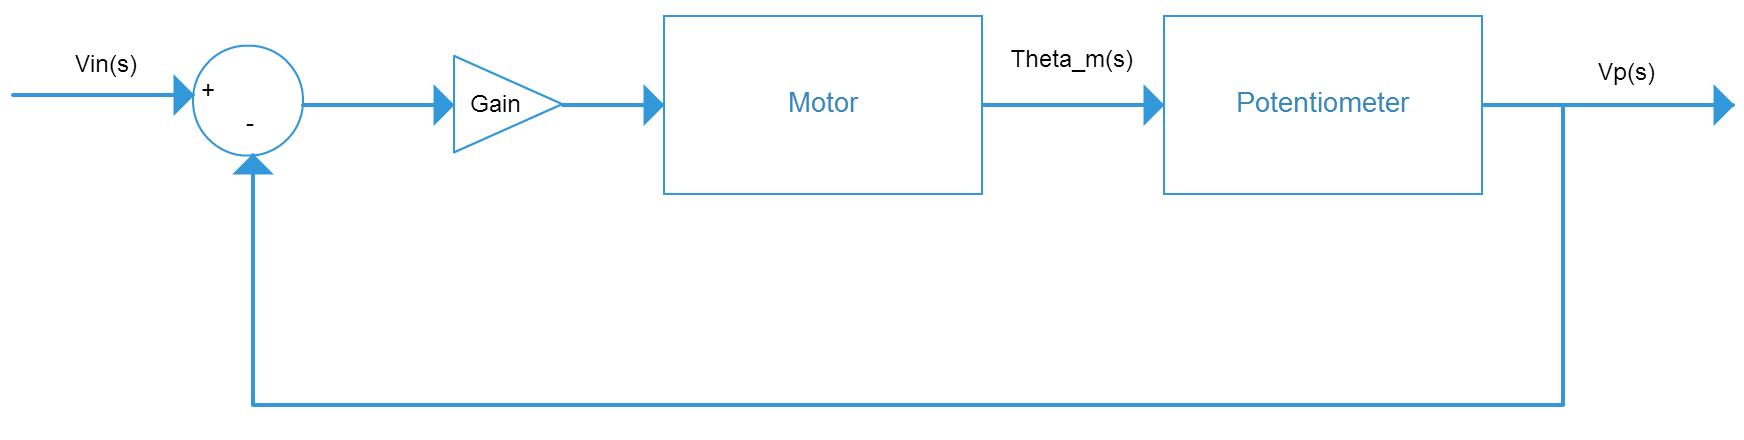
\includegraphics[width=.8\textwidth]{PreLach/A2a.png}
	\caption{\label{fig:funcagram}Functional Diagram of the control system}
	\end{figure}
    
    
	\item The updated functional diagram has been included below.
    \begin{figure}[H]
	\centering
	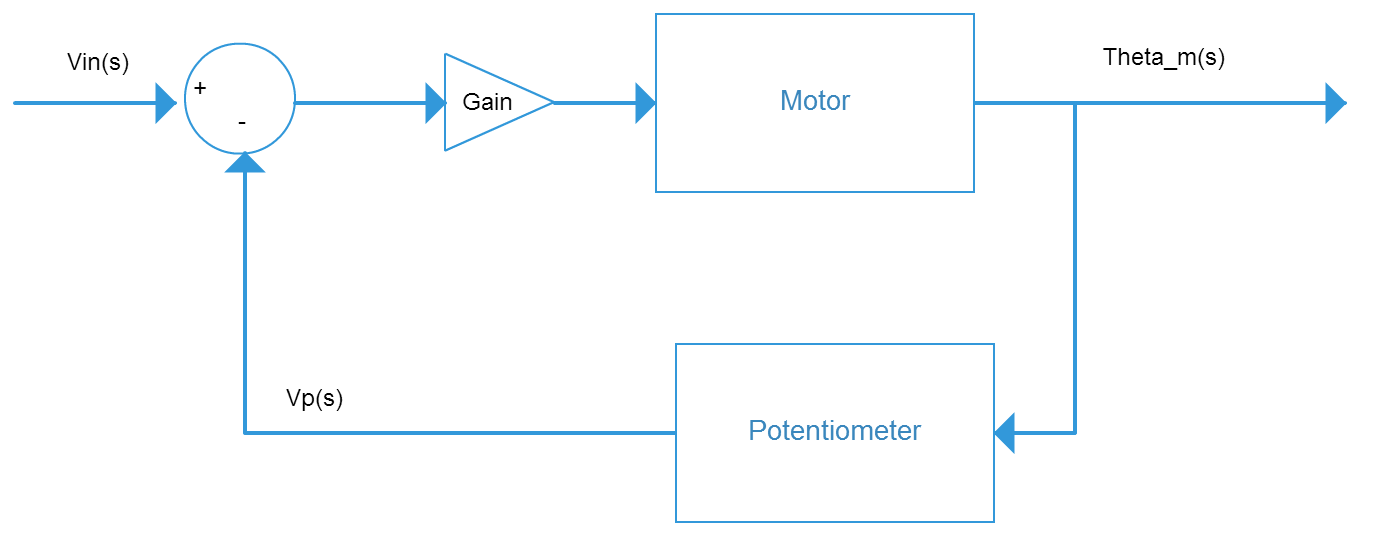
\includegraphics[width=.8\textwidth]{PreLach/A2b.png}
	\caption{\label{fig:updatedfuncagram}Updated Functional Diagram}
	\end{figure}
    
    
    
    
    \pagebreak
	\item The output of the requested matlab script has been included below, after which, the code itself has been provided. 
    \begin{figure}[H]
	\centering
	\includegraphics[width=.8\textwidth]{PreLach/a3.eps}
	\caption{\label{fig:simrep} Simulated Response}
	\end{figure}
    \begin{lstlisting}
%% A3
Alpha = 1;
K_m = 1;

t = linspace(0,10,100);
G_0 = tf([K_m],[1 Alpha 0]);
figure();
step(G_0, t, 'r')
print('-depsc','a3')
	\end{lstlisting}
    
    
    
    
    \pagebreak
	\item The given data describing the step response of an ideal servo model has been compared to the previously estimated system response. 
    \begin{figure}[H]
	\centering
	\includegraphics[width=.8\textwidth]{PreLach/a4.eps}
	\caption{\label{fig:datacomp}Given Data and Estimated Response}
	\end{figure}
    \begin{lstlisting}
%% A4    
Alpha = 1;
K_m = 1;
t = linspace(0,10,100);
G_0 = tf([K_m],[1 Alpha 0]);
    
load ENB301TestData_2015.mat
figure();
plot(t,y1);
hold;
step(G_0, t, 'r')
print('-depsc','a4')
	\end{lstlisting}
  
  
  
  
  
    \item \textbf{steady/transient Q}
    
    
    
    
    \pagebreak
    \item After changing the values of $K_m$ and $\alpha$ in the previous matlab script, it was found that values of $K_m = 1.3$ and $\alpha = 1$ resulted in an output that matched the test data. Furthermore, a script was created specifically to automatically find the best estimates for values of $K_m$ and $\alpha$ within a given range. The results of both the manual and automatic estimations have been included below. 
    \begin{figure}[H]
	\centering
	\includegraphics[width=.8\textwidth]{PreLach/a6a.eps}
	\caption{\label{fig:manest}Manually Estimated System Values}
	\end{figure}
    \begin{lstlisting}
%% A6
Alpha = 1; %0.5-1.5
K_m = 1.3; %1-2
G_0 = tf([K_m],[1 Alpha 0]);
figure();
plot(t,y1);
hold;
step(G_0, t, 'r');
print('-depsc','a6a')
	\end{lstlisting}
    
    \begin{figure}[H]
	\centering
	\includegraphics[width=.8\textwidth]{PreLach/a6b.eps}
	\caption{\label{fig:autoest}Inverting Amplifier System}
	\end{figure}
    \begin{lstlisting}
%% Automated:
% loop values of alpha and k_m
% calculate RMS error each time
% pick values with the least error

y1_rms = rms(y1);
prevdiff = 10000;

for Alpha = 0.1:0.1:3
    for K_m = 0.1:0.1:3
        G_0 = tf([K_m],[1 Alpha 0]);
        G_t = step(G_0, t, 'r');
        Gt_rms = rms(G_t);
        diff = y1_rms - Gt_rms;
        if (abs(diff) < abs(prevdiff))
            prevdiff = diff;
            K_m_f = K_m;
            Alpha_f = Alpha;
        end
    end
end

G_0 = tf([K_m_f],[1 Alpha_f 0]);
figure();
plot(t,y1);
hold;
step(G_0, t, 'r');
print('-depsc','a6b')

% Final values:
% Alpha_f = 1.3
% K_m_f = 1.7
    \end{lstlisting}
    
    
    
    
    
    
    \pagebreak
    \item Using matlabs random number generator, uncertainty was added to the output $y_1(t)$, and both the ideal and noisy response were plotted. \textbf{QUESTIONS}
    \begin{figure}[H]
	\centering
	\includegraphics[width=.8\textwidth]{PreLach/a7.eps}
	\caption{\label{fig:rand}Estimated System Response + Uncertainty}
	\end{figure}
    \begin{lstlisting}
%% A7
rand_power = 2;

y_1 = step(G_0, t, 'r');
y_n = y_1 + (rand_power/2)*rand(size(y_1,1),1) - (rand_power/2)*rand(size(y_1,1),1);

figure();
step(G_0, t, 'b');
hold;
plot(t,y_n,'r');
print('-depsc','a7')

	\end{lstlisting}
    
\end{enumerate}








\pagebreak
\subsubsection{Declan Gilmour}
\begin{enumerate}
	\item
	\item
	\item
	\item
\end{enumerate}










\pagebreak
\subsection{Answers:}
\subsubsection{Part B}
\begin{enumerate}
	\item Read experimental data file(s) and store in vectors $y_e(t)$ and $t_e$. Plot the experimental results in black.
    
    \begin{lstlisting}
%% B1
% Load experimental data and plot in black
data = csvread('PartB_Test1.csv',2,0);  % Read in test 1
te_1 = data(1:end,1);   % Store te variable
te_1 = te_1 + abs(te_1(1)); % Move te variable to start at zero
ye_1 = data(1:end,2);   % Store ye variable
ye_1step = data(1:end,3);   % Store ye step input variable

figure
plot(te_1,ye_1,'k',te_1,ye_1step,'b')   % Plot ye in black and ye in blue
title('Experimental Data Plot [Set 1]')
xlabel('te (sec)')
ylabel('ye (voltage)')
print('-depsc',strcat('figures',filesep,'B1_dataset1'));    % Store figure
close
    \end{lstlisting}

	
    
  \begin{figure}[h]
	
  \begin{subfigure}{0.5\textwidth}
  \includegraphics[width=0.9\linewidth]{Matlab_Figures/B1_dataset1.eps} 
  \caption{Data Set 1}
  \label{fig:subim1}
  \end{subfigure}
  \begin{subfigure}{0.5\textwidth}
  \includegraphics[width=0.9\linewidth]{Matlab_Figures/B1_dataset2.eps}
  \caption{Data Set 2}
  \label{fig:subim2}
  \end{subfigure}
  
  \begin{subfigure}{0.5\textwidth}
  \includegraphics[width=0.9\linewidth]{Matlab_Figures/B1_dataset3.eps}
  \caption{Data Set 3}
  \label{fig:subim3}
  \end{subfigure}

  \caption{\label{fig:rand}Open Loop response}
  \end{figure}

\pagebreak
	\item Modify the MATLAB script created in the pre-labs to simultaneously plot both the experimental data and $y_1(t)$.
    No real idea what to put here...
	\item Derive a figure of merit for the estimation compared with experimental results.
    \\Mean Square error calculation: $error = (G_0 - y_e)^2$
    \\Root Mean Square error calculation: $error = \sqrt[2]{(G_0 - y_e))^2}$
	\item Improve estimates using the plots and figure of merit calculations. Derive the two parameters for the servo motor function $G(s) = \frac{K_m}{(S + \alpha)(S + \beta)}$.
  \begin{figure}[H]
	
  \begin{subfigure}{0.5\textwidth}
  \includegraphics[width=0.9\linewidth]{Matlab_Figures/B2_dataset1.eps} 
  \caption{Data Set 1}
  \label{fig:subim1}
  \end{subfigure}
  \begin{subfigure}{0.5\textwidth}
  \includegraphics[width=0.9\linewidth]{Matlab_Figures/B2_dataset2.eps}
  \caption{Data Set 2}
  \label{fig:subim2}
  \end{subfigure}
  
  \begin{subfigure}{0.5\textwidth}
  \includegraphics[width=0.9\linewidth]{Matlab_Figures/B2_dataset3.eps}
  \caption{Data Set 3}
  \label{fig:subim3}
  \end{subfigure}

  \caption{\label{fig:rand}Servo Motor Response Modified: $k_m$ and $\alpha$}
  \end{figure}
    
    \begin{lstlisting}
% Plot experimental data ye against systems estimated tf y1
[te_1new,ye_1new] = timing_fix(te_1,ye_1);
[te_2new,ye_2new] = timing_fix(te_2,ye_2);
[te_3new, ye_3new] = timing_fix(te_3,ye_3);

figure
plot(te_1new,ye_1new,'k')
title('Experimental Data Plot [Set 1 Adjusted]')
xlabel('te (sec)')
ylabel('ye (voltage)')
print('-depsc',strcat('figures',filesep,'B2_dataset1'));
close

figure
plot(te_1new,ye_1new,'k')
title('Experimental Data Plot [Set 1 Adjusted]')
xlabel('te (sec)')
ylabel('ye (voltage)')
print('-depsc',strcat('figures',filesep,'B2_dataset1'));
close
	\end{lstlisting}
	
    \begin{lstlisting}
% Pepare experimental data for alpha and km parameter calculations
[te_1trim, ye_1trim] = trimForCalculation(te_1new,ye_1new,mf1);
[te_2trim, ye_2trim] = trimForCalculation(te_2new,ye_2new,mf1);
[te_3trim, ye_3trim] = trimForCalculation(te_3new,ye_3new,mf1);

km_num = 500;    % number of km values used
km_max = 500;   % max km value used
alpha_num = 500;    % number of alpha values used
alpha_max = 500;    % max alpha value used
	\end{lstlisting}
\pagebreak    
    \begin{lstlisting}
% Preallocate size for speed
output_ms = zeros(3,km_num*alpha_num);
output_rms = zeros(3,km_num*alpha_num);
km_ms = zeros(1,3);
alpha_ms = zeros(1,3);
km_rms = zeros(1,3);
alpha_rms = zeros(1,3);
        
for iteration = 1 : 3
    
    % Set te and ye based on iteration
    if (iteration == 1)        
        te = te_1trim;
        ye = ye_1trim;
    elseif (iteration == 2)
        te = te_2trim;
        ye = ye_2trim;
    else
        te = te_3trim;
        ye = ye_3trim;
    end      
    
    % Set cycle variables
    error_ms = 0;
    error_rms = 0;
    ii = 1;
    count = 0;
    
    for km = linspace(0,km_max,km_num)   % Cycle km values
       for alpha = linspace(0,alpha_max,alpha_num)  % Cycle alpha values
           G = tf(km, [1 alpha 0]);
           G_0 = step(G,te);

           % Calculate error
           for jj = 1 : length(te)
              % Calculate mean square error
              error_ms = error_ms + (G_0(jj) - ye(jj))^2;
              
              % Calculate root mean square error
              error_rms = error_rms + rms(G_0(jj) - ye(jj));
           end
           
           % Store km, alpha and the error taken to calculate
           output_ms(:,ii) = [km;alpha;error_ms];
           output_rms(:,ii) = [km;alpha;error_rms];
           
           % Reset cycle variables
           ii = ii + 1;
           error_ms = 0;
           error_rms = 0;
       end
       
       % Output km iterations
       %count = count + 1;       
       %fprintf('%d %s %d\n',count,'/',km_num);
    end

    % Calculate km and alpha values for mean square error calculation
    [~,index] = min(output_ms(3,:));
    km_ms(iteration) = output_ms(1,index); % Output variable
    alpha_ms(iteration) = output_ms(2,index);  % Output variable

    % Calculate km and alpha values for root mean square error calculation
    [~,index] = min(output_rms(3,:));
    km_rms(iteration) = output_rms(1,index); % Output variable
    alpha_rms(iteration) = output_rms(2,index);  % Output variable    
end
km_mean = (mean(km_ms) + mean(km_rms)) / 2;
alpha_mean = (mean(alpha_ms) + mean(alpha_rms)) / 2;
    \end{lstlisting}
    
    \begin{lstlisting}
% Plot y1 against ye
% Data Set 1
G = tf(km_ms(1), [1 alpha_ms(1) 0]);
y1_ms = step(G,te_1new);
figure
plot(te_1new,medfilt1(ye_1new,1),'k',te_1new,medfilt1(y1_ms,1),'b')
title('Experimental vs estimated TF [Set 1 Adjusted, mean square error]')
xlabel('te (sec)')
ylabel('y (voltage)')
legend('ye','y1')
print('-depsc',strcat('figures',filesep,'y1_dataset1_ms'));
close
    \end{lstlisting}
    The average constants found are as follows:
    $\alpha = 170.3407$
    $k_m = 422.0107$
    
   \begin{figure}[H]
	
  \begin{subfigure}{0.5\textwidth}
  \includegraphics[width=0.9\linewidth]{Matlab_Figures/y1_dataset1_ms.eps} 
  \caption{Data Set 1 (ms)}
  \label{fig:subim1}
  \end{subfigure}
  \begin{subfigure}{0.5\textwidth}
  \includegraphics[width=0.9\linewidth]{Matlab_Figures/y1_dataset1_rms.eps}
  \caption{Data Set 1 (rms)}
  \label{fig:subim2}
  \end{subfigure}
  
  
  \begin{subfigure}{0.5\textwidth}
   \includegraphics[width=0.9\linewidth]{Matlab_Figures/y1_dataset2_ms.eps} 
   \caption{Data Set 2 (ms)}
   \label{fig:subim1}
   \end{subfigure}
   \begin{subfigure}{0.5\textwidth}
   \includegraphics[width=0.9\linewidth]{Matlab_Figures/y1_dataset2_rms.eps}
   \caption{Data Set 2 (rms)}
   \label{fig:subim2}
   \end{subfigure}
  
   \begin{subfigure}{0.5\textwidth}
   \includegraphics[width=0.9\linewidth]{Matlab_Figures/y1_dataset3_ms.eps} 
   \caption{Data Set 3 (ms)}
   \label{fig:subim1}
   \end{subfigure}
   \begin{subfigure}{0.5\textwidth}
   \includegraphics[width=0.9\linewidth]{Matlab_Figures/y1_dataset3_rms.eps}
   \caption{Data Set 3 (rms)}
   \label{fig:subim2}
   \end{subfigure}
   \caption{\label{fig:rand}Servo Motor Response Modeled}
   \end{figure}
	\item The mechanical constant $\alpha$ was found to be $\alpha = alpha_{mean}$. Using the second order equation $G(s) = \frac{K_m}{(S + \alpha)}$ new values of gain constant $k_m$ and electrical constant $\beta$. Values were found for $y_1(t) \approx y_2(t)$.
    The average constants found are as follows:
    $\beta = 0.0646$
    $k_m = 426.6867$
    
   \begin{figure}[h]
	
  \begin{subfigure}{0.5\textwidth}
  \includegraphics[width=0.9\linewidth]{Matlab_Figures/y2_dataset1_ms.eps} 
  \caption{Data Set 1 (ms)}
  \label{fig:subim1}
  \end{subfigure}
  \begin{subfigure}{0.5\textwidth}
  \includegraphics[width=0.9\linewidth]{Matlab_Figures/y2_dataset1_rms.eps}
  \caption{Data Set 1 (rms)}
  \label{fig:subim2}
  \end{subfigure}
  
  
 \begin{subfigure}{0.5\textwidth}
  \includegraphics[width=0.9\linewidth]{Matlab_Figures/y2_dataset2_ms.eps} 
  \caption{Data Set 2 (ms)}
  \label{fig:subim1}
  \end{subfigure}
  \begin{subfigure}{0.5\textwidth}
  \includegraphics[width=0.9\linewidth]{Matlab_Figures/y2_dataset2_rms.eps}
  \caption{Data Set 2 (rms)}
  \label{fig:subim2}
  \end{subfigure}
  
  \begin{subfigure}{0.5\textwidth}
  \includegraphics[width=0.9\linewidth]{Matlab_Figures/y2_dataset3_ms.eps} 
  \caption{Data Set 3 (ms)}
  \label{fig:subim1}
  \end{subfigure}
  \begin{subfigure}{0.5\textwidth}
  \includegraphics[width=0.9\linewidth]{Matlab_Figures/y2_dataset3_rms.eps}
  \caption{Data Set 3 (rms)}
  \label{fig:subim2}
  \end{subfigure}
    \caption{\label{fig:rand}Servo Motor Response Modeled: $k_m$ and $\beta$}
    \end{figure}
    
 \begin{lstlisting}
km_num = 500;    % number of km values used
km_max = 500;   % max km value used
beta_num = 50;    % number of alpha values used
beta_max = 1;    % max alpha value used

% Preallocate size for speed
output_ms = zeros(3,km_num*beta_num);
output_rms = zeros(3,km_num*beta_num);
km2_ms = zeros(1,3);
beta_ms = zeros(1,3);
km2_rms = zeros(1,3);
beta_rms = zeros(1,3);
    
for iteration = 1:3
    if(iteration == 1)
        te = te_1trim;
        ye = ye_1trim;
    elseif(iteration==2)
        te = te_2trim;
        ye = ye_2trim;
    else
        te = te_3trim;
        ye = ye_3trim;
    end
    
    % Set cycle variables
    error_ms = 0;
    error_rms = 0;
    ii = 1;
    count = 0;
    
    for km = linspace(0,km_max,km_num)   % Cycle km values
       for beta = linspace(0,beta_max,beta_num)  % Cycle alpha values
           G = tf(km, [1 (alpha_mean+beta) (alpha_mean*beta)]);
           G_0 = step(G,te);

           % Calculate error
           for jj = 1 : length(te)
              % Calculate mean square error
              error_ms = error_ms + (G_0(jj) - ye(jj))^2;

              % Calculate root mean square error
              error_rms = error_rms + rms(G_0(jj) - ye(jj));
           end

           % Store km, alpha and the error taken to calculate
           output_ms(:,ii) = [km;beta;error_ms];
           output_rms(:,ii) = [km;beta;error_rms];

           % Reset cycle variables
           ii = ii + 1;
           error_ms = 0;
           error_rms = 0;
       end

        % Output km iterations
       %count = count + 1;       
       %fprintf('%d %s %d\n',count,'/',km_num);
    end

    % Calculate km and alpha values for mean square error calculation
    [~,index] = min(output_ms(3,:));
    km2_ms(iteration) = output_ms(1,index); % Output variable
    beta_ms(iteration) = output_ms(2,index);  % Output variable

    % Calculate km and alpha values for root mean square error calculation
    [~,index] = min(output_rms(3,:));
    km2_rms(iteration) = output_rms(1,index); % Output variable
    beta_rms(iteration) = output_rms(2,index);  % Output variable 
end

km_mean2 = (mean(km_ms) + mean(km2_rms)) / 2;
beta_mean = (mean(beta_ms) + mean(beta_rms)) / 2;
    \end{lstlisting}
    
    \begin{lstlisting}
% Plot y2 against ye
% Data Set 1
G = tf(km2_ms(1), [1 (alpha_mean+beta_ms(1)) (alpha_mean*beta_ms(1))]);
y2_ms = step(G,te_1new);
figure
plot(te_1new,medfilt1(ye_1new,1),'k',te_1new,medfilt1(y2_ms,1),'b')
title('Experimental vs estimated TF [Set 1 Adjusted, mean square error]')
xlabel('te (sec)')
ylabel('y (voltage)')
legend('ye','y1')
print('-depsc',strcat('figures',filesep,'y2_dataset1_ms'));
close
    \end{lstlisting}
    
\end{enumerate}













\pagebreak
\subsubsection{Part C}
\label{sec:c}
\begin{enumerate}
	\item \textbf{Re-draw figure~\ref{fig:c1_2_} and place boxes around the set of components that  correspond to each functional element of the control system.} \\
    
	\begin{figure}[H]
	\centering
	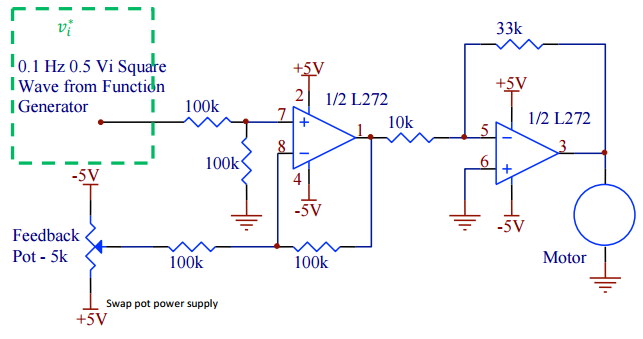
\includegraphics[width=.8\textwidth]{FigsC/c1_2_.png}
	\caption{\label{fig:c1_2_}Closed Loop Motor Control Schematic}
	\end{figure}
    
    \begin{figure}[H]
	\centering
	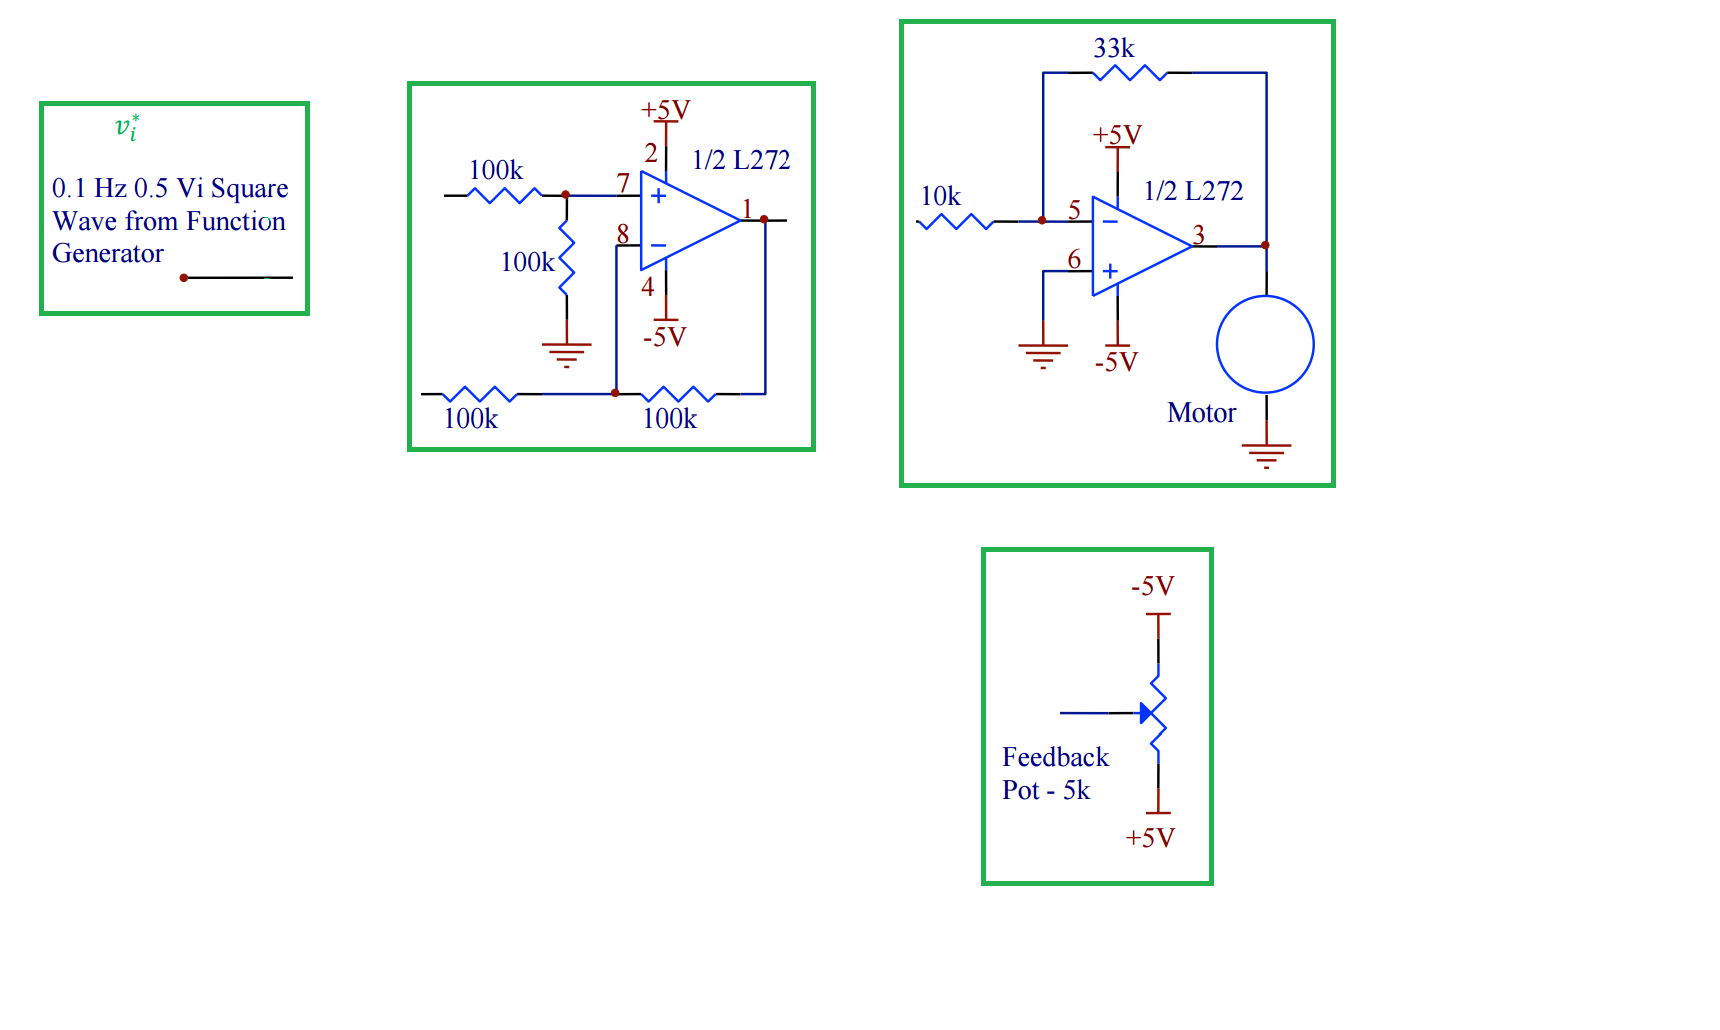
\includegraphics[width=.8\textwidth]{FigsC/c1.png}
	\caption{\label{fig:c1}Closed Loop Motor Control System}
	\end{figure}
    
    
    
    
    
    \pagebreak
	\item \textbf{Based on the results from Parts A and B, the component values given in figure~\ref{fig:c1_2_} and your research in parts C1, calculate all of the transfer functions in your functional diagram (figure~\ref{fig:c1}). Update the functional diagram, labeling all components and interfaces.}  \\
    
    \textbf{Difference Op-amp:}\\
    \begin{figure}[H]
	\centering
	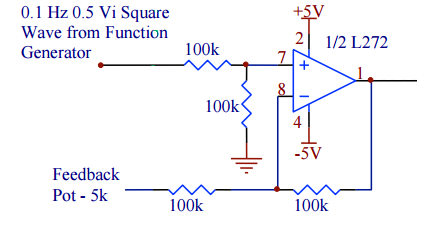
\includegraphics[width=.4\textwidth]{FigsC/c2b.png}
	\caption{\label{fig:diffamp}Difference Op-amp System}
	\end{figure}
    \begin{align*}
	\frac{V_{1}(s)}{V_{in}(s)} &= V_{in}(s) - V_{p}(s)
	\end{align*}
    
    
    \textbf{Inverting Op-amp:}\\
    \begin{figure}[H]
	\centering
	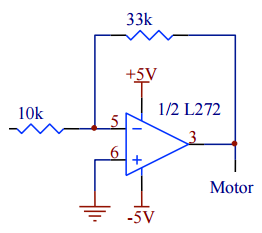
\includegraphics[width=.3\textwidth]{FigsC/c2a.png}
	\caption{\label{fig:invamp}Inverting Amplifier System}
	\end{figure}
    \begin{align*}
	\frac{V_{m}(s)}{V_{1}(s)} &= \frac{R_2}{R_1}
	\end{align*}
    
    
    \textbf{Motor and pot:}\\
    \begin{align*}
	\frac{V_{p}(s)}{V_{m}(s)} &= \frac{K_m}{s(s+\alpha)}
	\end{align*}
    
    something \\
    
    
    
    \pagebreak
	\item 
    \textbf{NONIDEAL:}\\
    \begin{align*}
	V_{m}(s) &= \frac{R_2}{R_1} V_{1}(s) \\
    V_{m}(s) &= \frac{s(s+\alpha)}{K_m} V_{p}(s) \\
    \frac{R_2}{R_1} V_{1}(s) &= \frac{s(s+\alpha)}{K_m} V_{p}(s) \\
    V_{1}(s) &= \frac{R_1 s(s+\alpha)}{R_2 K_m} V_{p}(s) \\
    V_{1} &= 
	\end{align*}
    
    
    
    
    
    \pagebreak
    \textbf{IDEAL:}\\
    \begin{align*}
    G_c(s) &= \frac{K G(S)}{1 + K G(s) H(s)} \\\\
    G(s) &= \frac{K_m}{s(s+\alpha)} \\
    H(s) &= 1 \\
    K &= \frac{R_f}{R_1} \\\\
    G_c(s) &= \frac{\frac{R_f}{R_1} G(s)} {1 + \frac{R_f}{R_1} G(s)} \\
    G_c(s) &= \frac{\frac{R_f}{R_1} \frac{K_m}{s(s+\alpha)}} {1 + \frac{R_f}{R_1} \frac{K_m}{s(s+\alpha)}} \\
    G_c(s) &= \frac{\frac{\frac{R_f}{R_1}K_m}{s(s+\alpha)}} {1 + \frac{\frac{R_f}{R_1}K_m}{s(s+\alpha)}} \\
    G_c(s) &= \frac{\frac{R_f}{R_1}K_m} {s(s+\alpha) + \frac{R_f}{R_1}K_m} \\
    G_c(s) &= \frac{\frac{R_f}{R_1}K_m} {s^2 + s\alpha + \frac{R_f}{R_1}K_m}
	\end{align*}
    
    Where $K_m = 326$, $\alpha = 38.61$, $R_f = 33k$ and $R_1 = 10k$.
    Thus,
    
    \begin{align*}
	G_c(s) &= \frac{\frac{33000}{10000}K_m} {s^2 + s\alpha + \frac{33000}{10000}K_m} \\
    G_c(s) &= \frac{3.3*K_m} {s^2 + s\alpha + 3.3*K_m} \\
    G_c(s) &= \frac{3.3*326} {s^2 + 38.61s + 3.3*326} \\
    G_c(s) &= \frac{1075.8} {s^2 + 38.61s + 1075.8} \\
	\end{align*}
    
    
    
    
    
    
    
    
    
    
	\item \textbf{\textcolor{red}{C4 - Matlab - Declan?}}
    
    
    
    
    
    
    
    
    \pagebreak
	\item \textbf{Calculate the gain required in the final stage to produce a 5\% overshoot. Choose resistor values to match the required gain.} \\\\
    Recall, for 5\% overshoot, $\zeta = \frac{-\ln(5/100)}{\sqrt[]{\pi^2+\ln^2(5/100)}} = 0.69$\\
    And, the systems estimated overall transfer function; $\frac{k_m\frac{R_f}{R_1}}{s^2 + s\alpha + k_m\frac{R_f}{R_1}}$\\
    Whereas, the general second order transfer function; $\frac{W_n^2}{s^2 + 2\zeta W_n s + W_n^2}$\\
    
    Moreover, 
    \begin{align*}
	\alpha &= 2\zeta W_n\\
    W_n &= \frac{\alpha}{2\zeta}
	\end{align*}
    \begin{align*}
	W_n^2 &= k_m\frac{R_f}{R_1}\\
    \frac{R_f}{R_1} &= W_n^2/k_m\\
    K &= (\frac{\alpha}{2\zeta})^2/k_m
	\end{align*}
    
    From section B, we know $k_m = 326$ and $\alpha = 38.61$. We also calculated the required $\zeta$ previously, as 0.69. 
    
    \begin{align*}
    K &= (\frac{38.61}{2*0.69})^2/326\\
    K &= 2.4
	\end{align*}
    
    Therefore, the gain required to achieve a 5\% overshoot is as stated above; Moreover, to calculate the desired resistor values to achieve this game, we must make an initial assumption about either $R_f$ or $R_1$. \\
    Assuming $R_1 = 10k$ (as to avoid changing both resistors);
    \begin{align*}
    K &= 2.4 \\
    \frac{R_f}{R_1} &= 2.4 \\
    R_f &= 2.4*R_1 \\
    R_f &= 2.4*10 000 \\
    R_f &= 24 000 
	\end{align*}
    
    Thus, theoretically, to achieve 5\% overshoot a gain of $K = 2.4$ is required, to achieve this, $R_f = 24k \approx 22k + 1.8k + 220 = 24.2k$, and $R_1 = 10k$. 
    
%     Moreover, $W_n = \sqrt[]{b}$, $\zeta = \frac{a}{2b}$
%     \begin{align*}
% 	\zeta &= \frac{\alpha}{2*k_m\frac{R_f}{R_1}}\\
%     \zeta &= \frac{\alpha}{\frac{2*k_m*R_f}{R_1}}\\
%     \zeta &= \frac{\alpha*R_1}{2*k_m*R_f}\\
%     \zeta &= \frac{\alpha}{2*k_m} * \frac{R_1}{R_f}\\
%     \frac{R_f}{R_1} &= \frac{\alpha}{2*k_m*\zeta}\\
% 	\end{align*}
    
%     From section B, we know $k_m = 326$ and $\alpha = 38.61$. We also calculated the required $\zeta$ previously, as 0.69. 
    
%     \begin{align*}
%     \frac{R_f}{R_1} &= \frac{38.61}{2*326*0.69}\\
%     \frac{R_f}{R_1} = K &= \frac{38.61}{2*326*0.69}\\
% 	\end{align*}

	
    
    
    
    
    
	\item \textbf{\textcolor{red}{C6 - Matlab - Declan?}}
    
    
    
    \pagebreak
	\item \textbf{Compare your experimentally derived 5\% overshot gain value against your predicted value. What is the percentage error? If your overshoot was too large for your derived gain value, could you use a controller other than the proportional controller to reduce overshoot? \\\\
If your steady state error was large, what other controller type could you use to minimize this error? What are  the drawbacks of  this  type of controller? What control applications can you think of that require very low steady state error?}\\

From the procedure outlined in \textbf{experiment C}, an experimental gain of $K = 6.28$ resulted in an overshoot of 5\%, and in \textbf{step 5} it was shown that the theoretical gain required to achieve this was $K = 2.4$. \\

Percentage error = blah \\

something \\

Steady state error \textbf{was} noticeable in the system, likely caused by mechanical losses (gearbox, heat, etc). To alleviate this issue, an PI compensator (integrator) could be used; this is because the controller adds up error over time, and would \textbf{know that it had still not yet reached the desired output}. Whereas, currently; the error signal of the proportional controller \textbf{does what?}.\\

Drawbacks/application? \\

Add the actual OS from prac/theo \\

    
    
    
    
    
    
    
	\item Another method of calculating TF? (bode)
\end{enumerate}










\pagebreak
\subsubsection{Part D}
\begin{enumerate}
	\item stuff
	\item comment
	\item gain
	\item simulink 
	\item PD/PI/PID controller 
\end{enumerate}











\section{SHIT}
NOTES:
on first page, acknowledge assistance from students 
list group members / lab members


%\subsection{Exercise Alpha}




\end{document}